\documentclass[a4paper,11pt,titlepage]{jarticle}
\usepackage[dvipdfmx]{graphicx}
\usepackage{listings}
\usepackage{amsmath}
\usepackage{fancybox,ascmac}

\title{知能情報実験I : 第三回レポート}
\author{175751C 宮城孝明}
\date{\today}

\begin{document}
\maketitle
\tableofcontents
\clearpage

\section{Task1}
\begin{figure}[htbp]
	\centering
	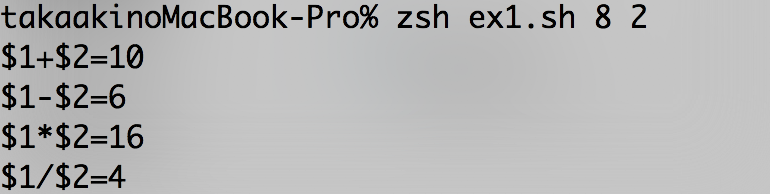
\includegraphics[width=100mm]{task3_1.png}
	\label{task3_1}\\
\end{figure}

\section{Task2}
\begin{figure}[htbp]
	\centering
	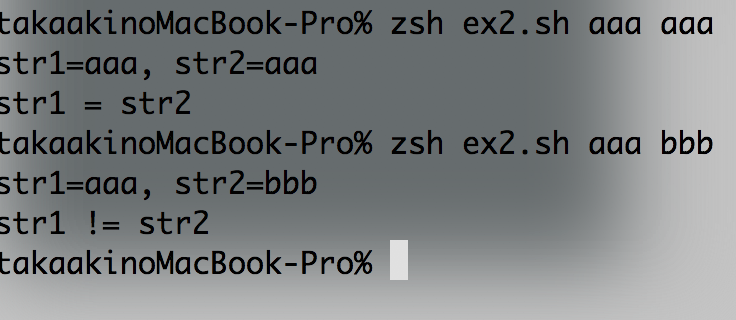
\includegraphics[width=100mm]{task3_2.png}
	\label{task3_2}\\
\end{figure}

\section{Task3}
\begin{figure}[htbp]
	\centering
	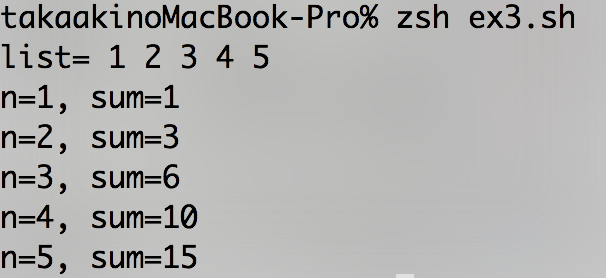
\includegraphics[width=100mm]{task3_3.png}
	\label{task3_3}\\
\end{figure}
\section{Task4}
\begin{figure}[htbp]
	\centering
	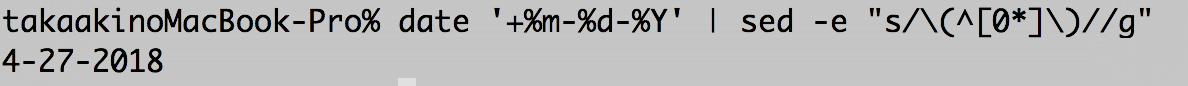
\includegraphics[width=120mm]{task3_4.png}
	\label{task3_4}\\
\end{figure}

\section{optiontask}
このスクリプトは、買い物中などに利用するために作成した。これで、買い物でいくら使うのかがわかる。
工夫したところは、0を入力したらループ処理を終了することである。0以外の数字だと値などがごちゃごちゃしてしまい、結果がおかしくなってしまうので、値に影響を及ぼさない0を起用した。
 \begin{figure}[htbp]
	\centering
	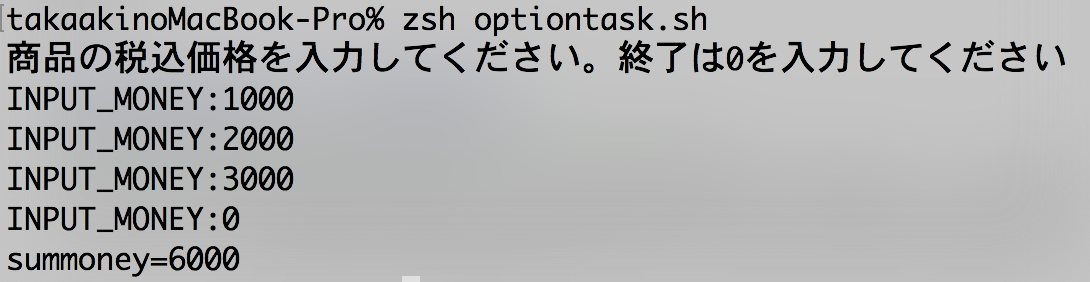
\includegraphics[width=100mm]{task3_5.png}
	\label{task3_5}\\
\end{figure}
\lstinputlisting[language=SH, numbers=left, breaklines=true, basicstyle=\ttfamily\footnotesize, frame=single, caption=サンプルプログラム, label=pg:optiontask]{optiontask.sh}
\section{specialtask}
\subsection{\TeX に関する調査検証}
 \TeX は、文書作成に適したソフトウェアであることは、この講義によって学んだ。主なメリットとしては、無料で使えることや、節の番号を自動設定してくれ、こちらはコードを書くことだけでいいのである。さらに、数式を綺麗に表現でき、数式に番号をつけられることも大きな要因として言えるだろう。一方、\TeX の中には、\LaTeX というのがある。\TeX の様々な命令を組み合わせて高機能な命令(マクロ)を作り、そのマクロを一通り揃えられたものをマクロ体系の一つを\LaTeX という。  
\subsection{gnuplotに関する調査検証}
 gnuplotとは、2次元や3次元のグラフを作成するためのアプリケーションである。インターネットで配布されており、多くのOSで利用可能でもある。オープンソフトウェアとして公開されており、高機能、高精度であるため、学術研究の際に用いられている。
 \begin{figure}[htbp]
	\centering
	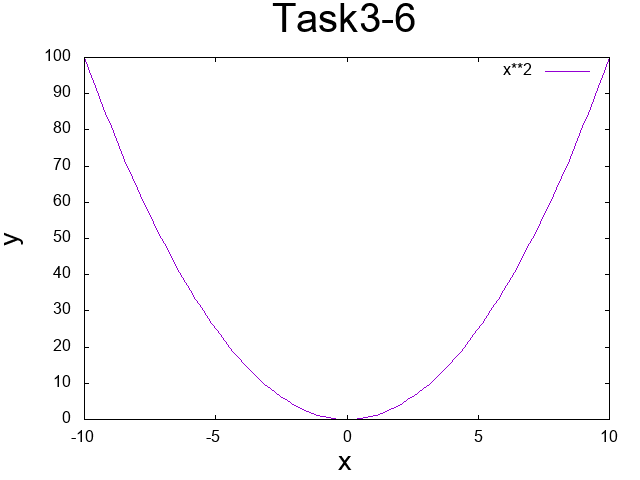
\includegraphics[width=125mm]{task3_6.png}
	\label{task3_6}\\
	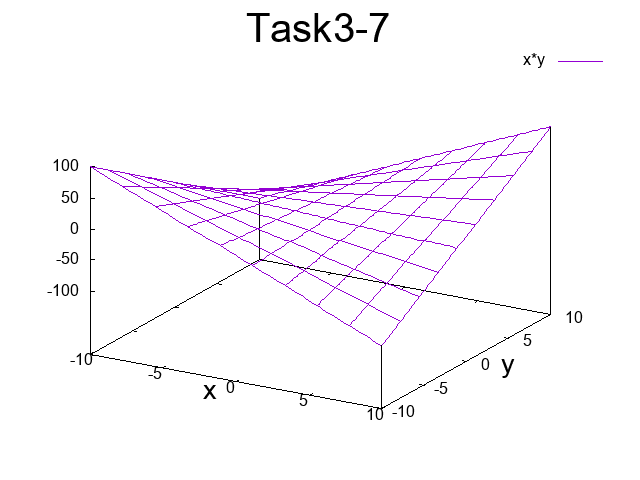
\includegraphics[width=125mm]{task3_7.png}
	\label{task3_7}\\
\end{figure}
\subsection{シェルスクリプト}
 シェルとは、OSとのやり取りをするためのインターフェースであり、コマンドを制御する」環境である。Linuxの核としているカーネル覆う殻がシェルとなる。もし、シェルがなければターミナルがどんなにコマンドを送ろうとうんともすんともしない。つまり、シェルとは、人間とカーネルの架け橋として活躍している。

\end{document}